%!TEX program = xelatex
% Note: this template must be compiled with XeLaTeX rather than PDFLaTeX
% due to the custom fonts used. The line above should ensure this happens
% automatically, but if it doesn't, your LaTeX editor should have a simple toggle
% to switch to using XeLaTeX.

\documentclass[
  aspectratio=169, % Uncomment to use an aspect ratio of 16:9 (160 mm by 90 mm)
  %aspectratio=43, % Uncomment to use an aspect ratio of 4:3 (128mm by 96mm)
  t, % Top align all slide content by default
  onlytextwidth, % Typeset content in columns at text width
  10pt, % Default font size, use 10pt for the 16:9 aspect ratio and 8pt for the 4:3 aspect ratio
]{beamer}

\usepackage{../../ImperialTheme/beamer/beamerthemeImperial} % Use the Imperial theme

\def\imagefolder{../../ImperialTheme/beamer/Images}

\title{Roughnesses in the domain} % Presentation title to appear on the title slide and left footers

\subtitle{} % Presentation subtitle to appear on the title slide

\author{Víctor Ballester} % Author name(s) to appear on the title slide

\date{\today} % Presentation date to appear on the title slide and right footers

\begin{document}

\begingroup
\setbeamercolor{background canvas}{bg=ICLBlue} % Slide background color
\setbeamercolor{title page title}{fg=white} % Title text color
\setbeamercolor{title page subtitle}{fg=white} % Subtitle text color
\setbeamercolor{author}{fg=white} % Author(s) text color
\setbeamercolor{date}{fg=white} % Date text color
\setbeamertemplate{title page}[logo]{\imagefolder/ICL_Logo_White.pdf} % Imperial logo color, use 'ICL_Logo_White.pdf' for white and 'ICL_Logo_Blue.pdf' for blue
\frame[plain, s]{\titlepage} % Output the title page with no footer ('plain') and vertically distributed text ('s')
\endgroup

\begin{frame}
  \frametitle{SVV vs no SVV (in SFD)}
  \begin{itemize}
    \item $w = 16.5\delta^*$  
    \item Plotted we show $|u_{SVV} - u_{no SVV}|$.
  \end{itemize}
  {
    \centering
    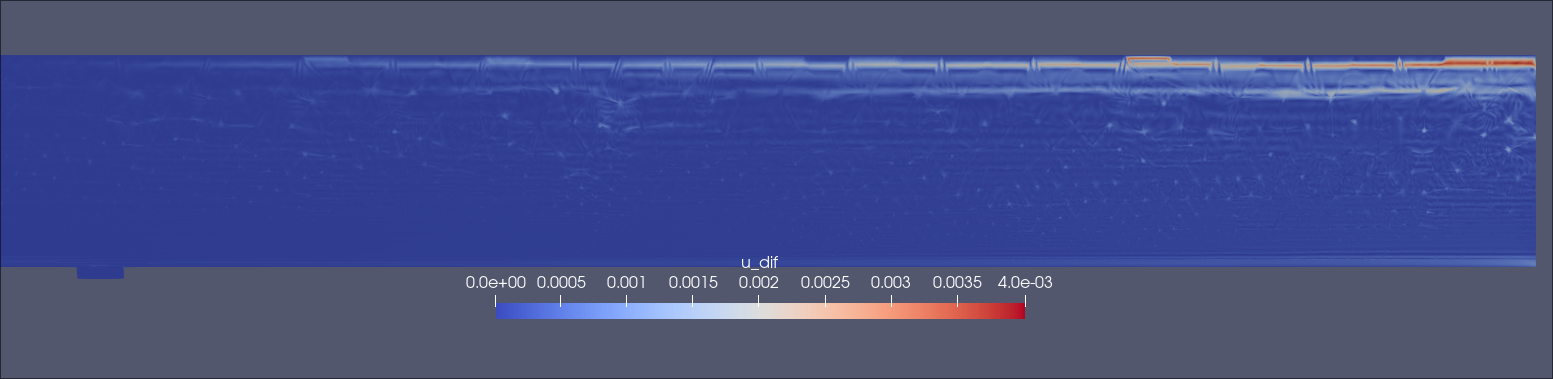
\includegraphics[width=0.95\textwidth]{Images/svv_full.png}
  }
\end{frame}
\begin{frame}
  {
    \centering
    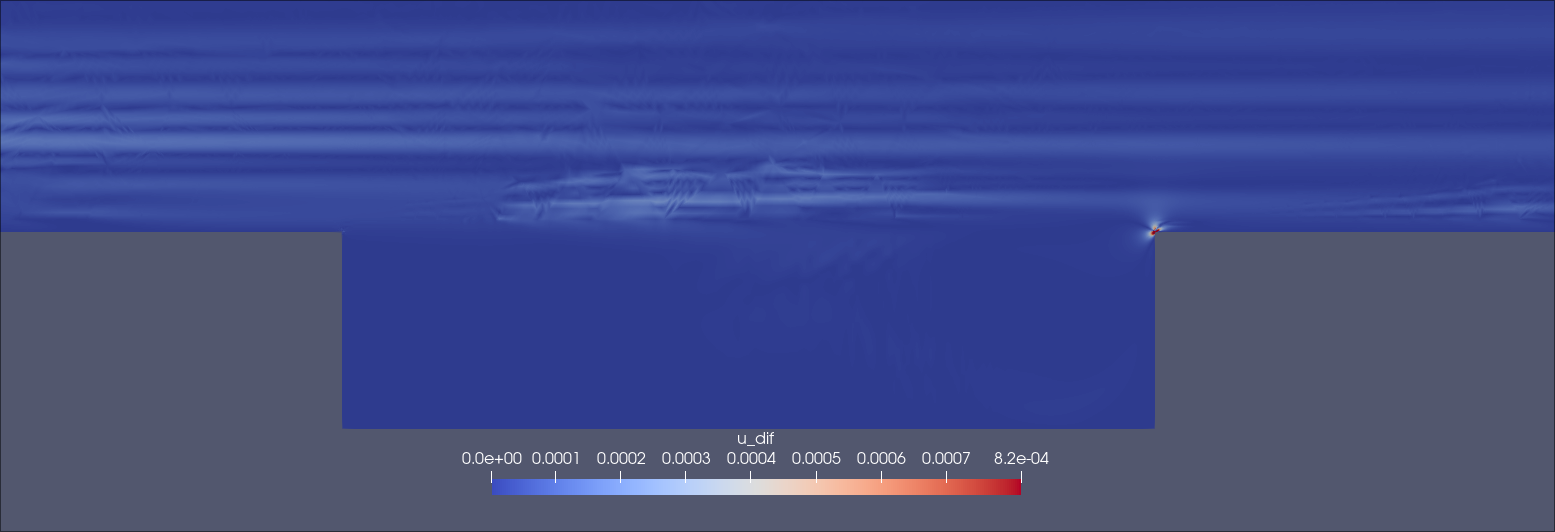
\includegraphics[width=0.95\textwidth]{Images/svv_gap.png}
  }
\end{frame}
\begin{frame}
  \frametitle{About SFD parameters}
  \begin{itemize}
  	\item I changed the filter width $\Delta$ from 2 to 4, but it is taken so long to converge. 
	  \begin{align*}
	    \dot{q} &= f(q) -\chi (q-\bar{q})\\
	    \dot{\bar{q}} &= \frac{q-\bar{q}}{\Delta}
	  \end{align*}
  \end{itemize}
\end{frame}
\begin{frame}
  \frametitle{Baseflow + eigenmode}
  {
    \centering
    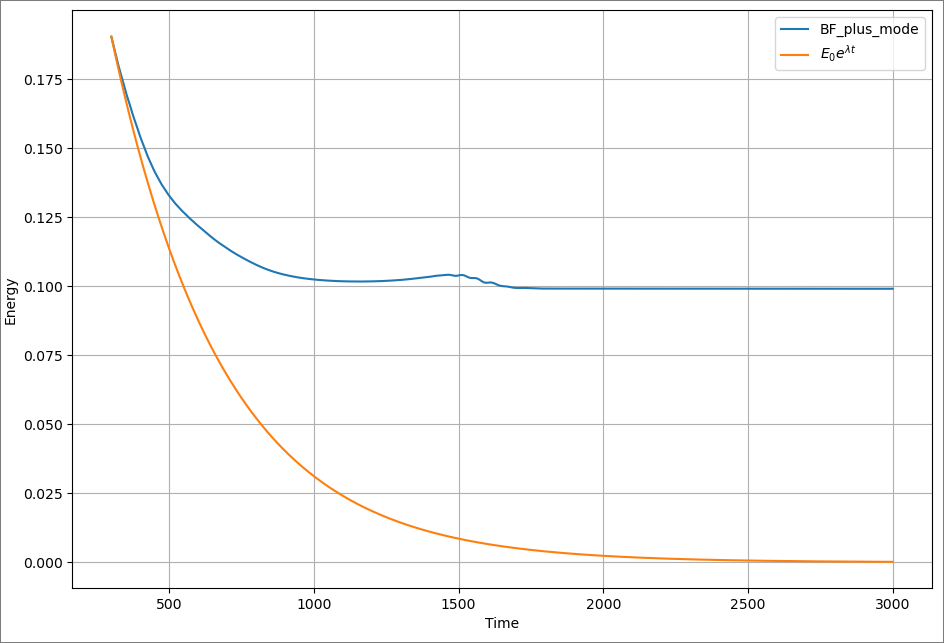
\includegraphics[width=0.5\textwidth]{Images/bf_u.png}

    L2 norm of the u-component (nonlinear vs linear theory).
  }

\end{frame}
\begin{frame}
  \frametitle{Baseflow + eigenmode}
  {
    \centering
    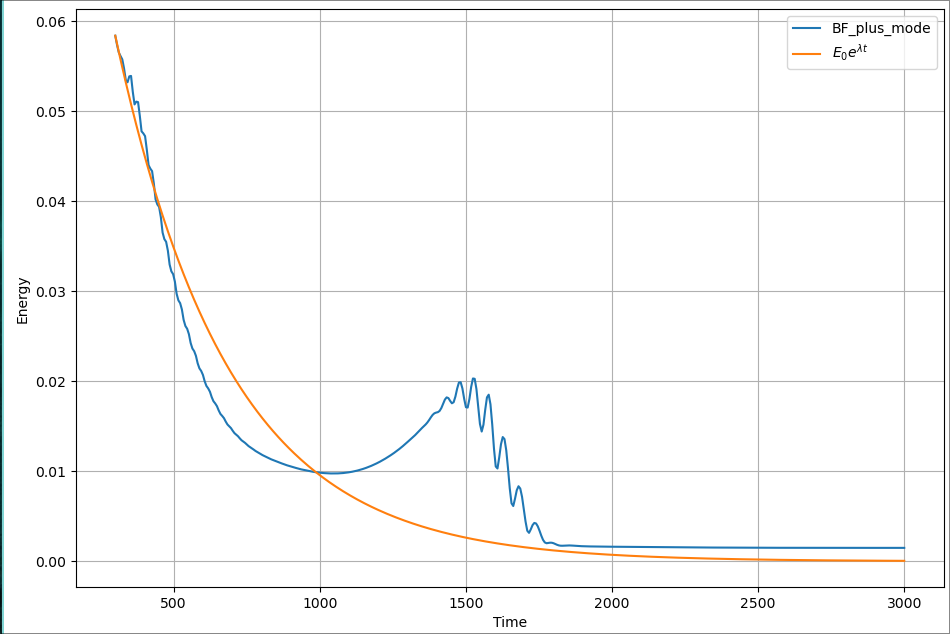
\includegraphics[width=0.5\textwidth]{Images/bf_v.png}

    L2 norm of the v-component (nonlinear vs linear theory).
  }

\end{frame}

\end{document}
